\documentclass[a4paper,10pt]{article}
\usepackage[utf8]{inputenc}
\usepackage{amsmath}
\usepackage{amsfonts}
\usepackage{amssymb}
\usepackage[german]{babel}
\setlength{\parindent}{0cm}
\usepackage{setspace}
\usepackage{mathpazo}
\usepackage{listings}
\usepackage{graphicx}
\usepackage{wasysym} 
\usepackage{booktabs}
\usepackage{verbatim}
\usepackage{ulem}
\usepackage{enumerate}
\usepackage{hyperref}
\usepackage{ulem}
\usepackage{stmaryrd }
\usepackage[a4paper,
left=1.8cm, right=1.8cm,
top=2.0cm, bottom=2.0cm]{geometry}
\usepackage{tabularx}
\usepackage{tikz}
\usetikzlibrary{trees,petri,decorations,arrows,automata,shapes,shadows,positioning,plotmarks}


\newcommand{\rf}{\right\rfloor}
\newcommand{\lf}{\left\lfloor}
\newcommand{\tabspace}{15cm}
\newcommand{\N}{\mathbb{N}}
\newcommand{\Z}{\mathbb{Z}}

\begin{document}
\begin{center}
\Large{Cognivite Algorithms: Assignment 2} \\
\end{center}
\begin{tabbing}
Tom Nick \hspace{2cm}\= - 340528\\
Maximilian Bachl \> - 341455 \\
\end{tabbing}

\begin{enumerate}
    \item The data set contains 2007 datapoints with each image having 256 pixels so one image is $16\cdot16$ pixels.
    \item Yes it does converge (just look at this magnificient graph). Because of the learning function, in the beginning more than in the end. \\
          \begin{center}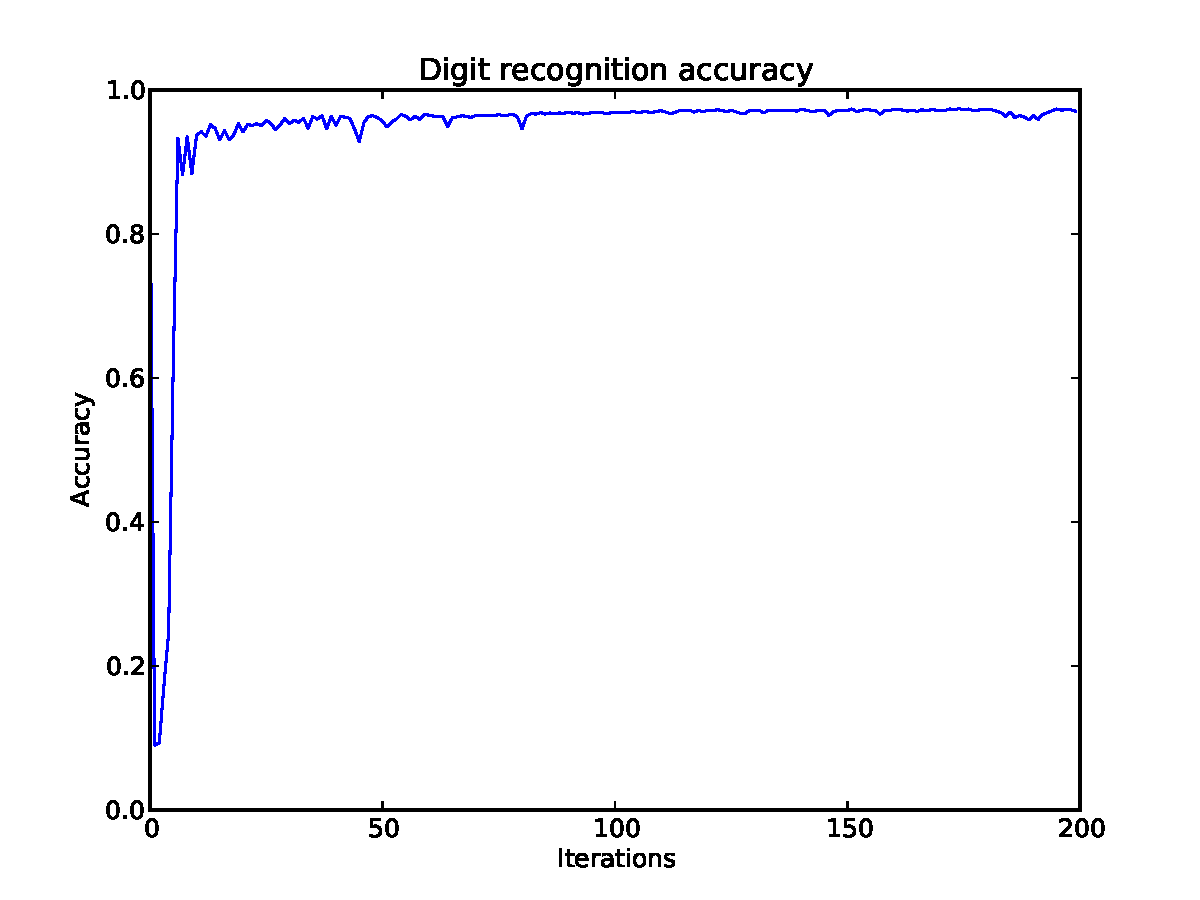
\includegraphics[scale=0.5]{./task_2_340528_341455.pdf}\end{center}
    \item[5.] I would certainly prefer the perceptron, because it's 1. has a higher accuracie and 2. the concept is much cooler.\\ \begin{center}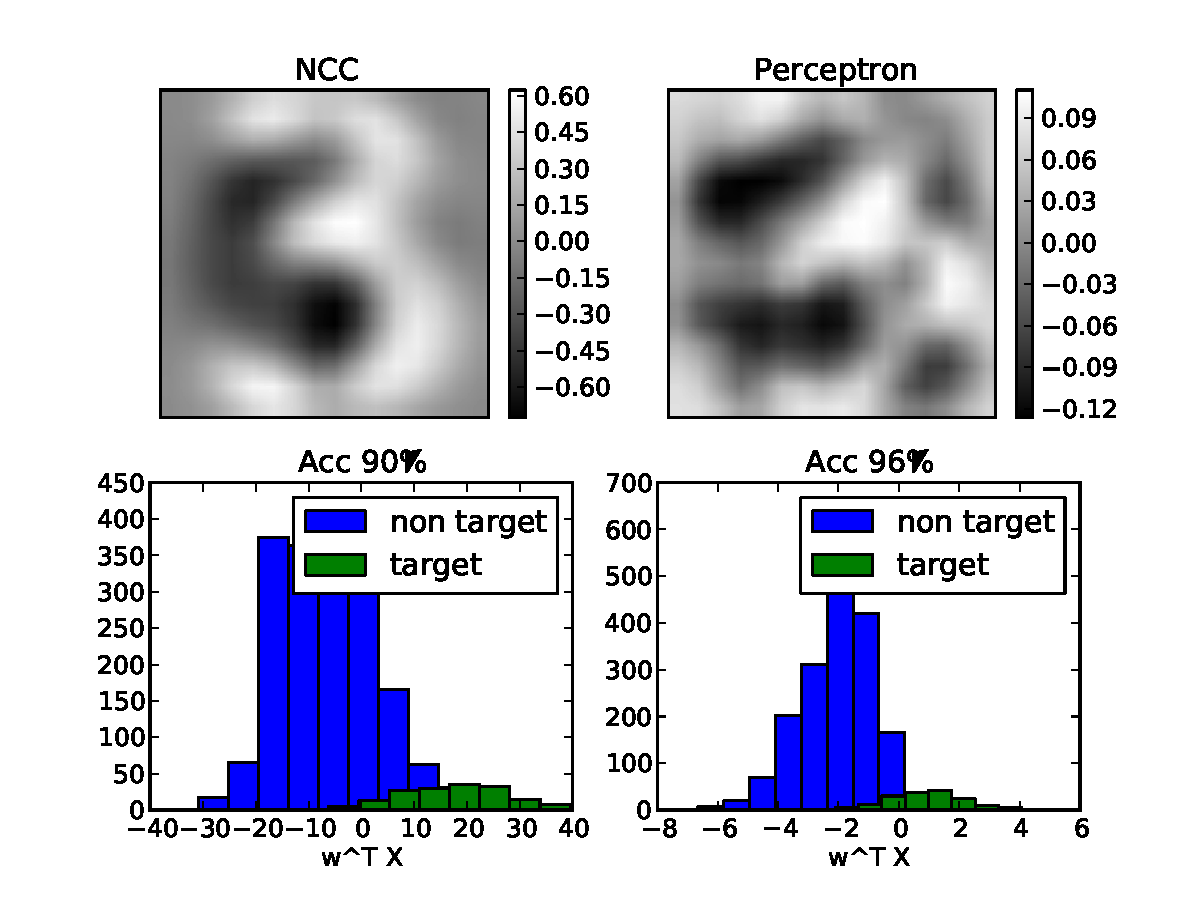
\includegraphics[scale=0.5]{./task_5_340528_341455.pdf}\end{center}
    \item[6.] It could be the case that we just had bad luck with the current data set. But generally the perceptron is probably better suited than the NCC for this kind of problem.
\end{enumerate}






\end{document}
